% CAS (Heimdall) -- system functional description, inlet system (water intake and pen level control)
% Structure after Cooling, Software Engineering for Real-Time Systems (2020), sec. 14.3 [COO].
\documentclass[11pt,a4paper]{article}
% amsmath defines \tag; casfd.sty redefines it as the instrument tag macro
\usepackage{amsmath}
\usepackage{casfd}
\usepackage{fancyhdr}
\usepackage{multicol}
\pagestyle{fancy}
\fancyhf{}
\lhead{\small CAS (Heimdall) -- FD inlet system}
\rhead{\small CAS-FD-10 rev.~B1}
\cfoot{\small\thepage}
\renewcommand{\headrulewidth}{0.3pt}
\setlength{\headheight}{14pt}
% let floats share pages with text instead of leaving half-empty pages
\renewcommand{\topfraction}{0.9}
\renewcommand{\bottomfraction}{0.8}
\renewcommand{\textfraction}{0.07}
\renewcommand{\floatpagefraction}{0.8}
\setcounter{totalnumber}{5}

\casfdheader{Inlet system: water intake and pen level control}{CAS-FD-10}{B}

% short helpers used only in this document
\newcommand{\TBD}{\textcolor{red}{TBD}}
\newcommand{\impl}{\textcolor{teal}{\textsf{yes}}}
\newcommand{\notimpl}{\textcolor{red}{\textsf{no}}}

\begin{document}
\maketitle
\thispagestyle{fancy}

\begin{abstract}
\noindent How the inlet system of the CAS (Heimdall) closed fish pen works and how the control system
controls it. Three Framo inlet pumps fill the pen with sea water; the Heimdall PLC holds the water inside
the pen a few centimetres above the sea outside (the \emph{over-height}) with one common pump speed, and
chooses how many pumps run. The
document covers every instrument and actuator, the control principle, sequences, the pump state machine,
interlocks, alarms and faults. Undecided points are marked \open{n} and listed in Section~\ref{sec:open}.
\end{abstract}

{\small\setlength{\parskip}{0pt}
\begin{multicols}{2}
\tableofcontents
\end{multicols}}

% =====================================================================================================
\section{Introduction}
\label{sec:intro}

\subsection{Purpose and readers}
The document is the system functional specification of the inlet system in the sense of
[COO]~\S14.3: a description of the physical system (\emph{block diagram description}), of what the
control system does with it (\emph{functional diagram description}) and of the functional and
non-functional requirements. It is written for
\begin{itemize}[nosep]
  \item \textbf{engineers and the project team}, who implement, test and commission the PLC program;
  \item \textbf{operators}, who need to know what the system does on its own and what they must do;
  \item \textbf{suppliers} (Framo for the inlet pumps), who must agree the interface and the behaviour
        at the boundary.
\end{itemize}
[FD] (Norwegian) is authoritative on the \emph{intent}. This document gives the intent in English,
shows what the PLC program [PLC] implements today (main, 2026-10-22) and where they differ.

\subsection{Scope}
\textbf{In scope:} the water intake from the three intakes to the pen (Framo inlet pumps PM-31/32/33,
their local controllers and vacuum systems as seen from the PLC), the level measurement inside and
outside the pen, the level controller LIC01, the start and stop of the pen and of each pump, the
communication with the Framo controllers and the related alarms.

\textbf{Out of scope} (separate FDs): the oxygen system (side stream, oxy pumps PU41--43, OIC01), the
outlet dampers and their hydraulics, the bilge system in the inlet boxes, and the power distribution.
They appear here only where they interface with the inlet system: the oxygenation permit per line,
the level setpoint per operating mode from the outlet, and interlocks from the inlet boxes.

\subsection{Sources}
\begin{table}[htbp]
\centering\small
\caption{Sources. The IDs are used in the text.}
\label{tab:sources}
\begin{tabularx}{\textwidth}{@{}P{17mm}LP{36mm}@{}}
\toprule
ID & Document & Revision / date \\
\midrule
{[FD]} & P-15169-CAS-FD-01 \emph{Funksjonsbeskrivelse CAS}, \S3.2.1 Vanninntak, \S3.2.2 level control,
  tables 5--10 (Norwegian) & rev.~B, 13.05.2026 \\
{[AL]} & P-15169-CAS-FD-02 \emph{Alarmliste CAS Heimdall} & rev.~A \\
{[FRAMO]} & Framo, \emph{Spesifikasjon: kontrollsystem (prototype)} 0000\_CAS\_SPEC\_CTRLSYS, signal list
  and state table, with ScaleAQ review comments & rev.~B, 08.10.2025 \\
{[FIL]} & Framo interface list (early signal list) & 01.09.2025 \\
{[PID]} & CAS P\&ID and loop diagrams: CAS-PID-100 inlet, -400 pen, -600 utilities, CAS-LAY-700
  network, CAS-LD-801 loop LT01, CAS-PID-950 open points & rev.~A, 2026-10-16 \\
{[DES]} & CAS design basis (System Modelling), generated from design\_basis.toml & v2.3.12 \\
{[PDS]} & CAS program design (dataflow of the level loop, start command path) & 2026-10-15 \\
{[PLC]} & Heimdall PLC program (CODESYS, application PFC200\_Sim): FB.Inlet.InletControl,
  InletSupervisor, InletSensors, FB.Pen.PenControl, PRG.FramoDataProcessing, GVL ConfigValues & main,
  2026-10-22 \\
{[EL]} & Electrical drawings 15169-792.001 (PLC/RIO1 cabinet), 792.002 (RIO2/3 cabinet),
  874.001 (Framo pump cabinet) & 792.001 rev.~1, 792.002 rev.~0 \\
{[COO]} & J.~Cooling, \emph{Software Engineering for Real-Time Systems}, 2020, \S14.3 System
  functional specifications & 2020 \\
\bottomrule
\end{tabularx}
\end{table}

\subsection{Abbreviations and terms}
\begin{small}
\begin{tabularx}{\textwidth}{@{}P{26mm}L@{}}
\toprule
Term & Meaning \\
\midrule
CAS & Closed Aquaculture System; Heimdall is the control system of the CAS pen \\
Over-height, $\Delta H$ & Water level inside the pen minus sea level outside [m or cm] \\
$\Delta H_i$, pair $i$ & Over-height measured at inlet $i$: LT0$i$ $-$ LT2$i$ \\
PV, SP & Process value, setpoint \\
LIC01 & Level indicating controller of the pen (PI) \\
Framo PCC$n$ & Pump control cabinet of inlet $n$: Beckhoff CX8200 PLC and ABB ACS880 drive \\
PFC200 & WAGO 750-8212, the Heimdall PLC \\
RIO & Remote I/O: WAGO 750-362 Modbus TCP couplers (CommonRIO, InletRIO1--3) \\
OPC UA & Communication between the PLC and the Framo controllers (and the HMI) \\
HMI & Operator interface (Heimdall HMI / SiteControl) \\
VSD & Variable speed drive \\
REMOTE, HOLD, \ldots & Pump states published by the Framo controller (Section~\ref{sec:sm}) \\
O-35, O-45, O-60, S-75 & Operating modes: operation (O) or service (S), with residence time in minutes \\
TBD & To be decided; see the open issues \\
\bottomrule
\end{tabularx}
\end{small}

\subsection{Revision note}
\begin{small}
\begin{tabularx}{\textwidth}{@{}P{10mm}P{22mm}L@{}}
\toprule
Rev. & Date & Change \\
\midrule
A & 2026-10-21 & First issue. Based on [FD] rev.~B, [FRAMO] rev.~B, [PID] rev.~A and the PLC branch in
  review (heartbeat, HOLD, per-pair PV and SafeOutput changes of 2026-10-15). Includes the review and
  simulator test of 2026-10-21. \\
A1 & 2026-10-21 & Reset to the PCC: held until the state change is seen, warning \emph{Failed to reset}
  after $2\times$\var{ResetExpectedTime}; HOLD$\to$REMOTE open issue reworded (the PLC follows the
  PCC either way); OI24 HMI Reset button. \\
B & 2026-10-22 & LIC01's output is the \emph{total} speed of the pumps in level control, shared by the pumps
  in REMOTE (Section~\ref{sec:lic}, DEC5; $K_p$ 1350 total rpm/m, one parameter set; OI5, OI6 closed).
  InletRIO link loss drops that inlet's pair (DEC6, OI17 closed). Level deviation alarms high/low (DEC8,
  OI8 in part). Automatic pump count and rotation by run time with \var{PumpCycleTime}
  (Section~\ref{sec:count}, DEC7, OI15 in part). Speed deviation alarm (OI9); LowPower / HighPower out of the
  common alarm (OI10 closed). Live test 2026-10-22 of the start, sharing, pump count and rotation
  (Section~\ref{sec:nfreq}). Operator commands restructured: pen state machine with Ready and pulses
  only, controller modes as pulses with a status, internal commands apart (Section~\ref{sec:seq}). Simulator
  tests of the sharing, the pump count, the rotation and the pen states are pending. \\
B1 & 2026-10-23 & LIC01 operator auto/manual bumpless both ways (IN-32): auto$\to$manual starts the manual
  output at the current output per pump (before, it jumped to the last \var{ManualOutput}, 40~rpm if
  never set); manual$\to$auto sets the setpoint to the PV and restarts with a cleared integral. Util.PID
  \var{RESET} / \var{Y\_OFFSET} use and the tuning-only-at-reset rule described (Section~\ref{sec:lic});
  the manual output is limited to the output range in \var{PIDController}. \\
\bottomrule
\end{tabularx}
\end{small}

% =====================================================================================================
\section{Block diagram description}
\label{sec:block}

\subsection{The process in brief}
The pen PEN01 is a closed bag of about 20\,000~m$^3$ (\O\,50.5~m, depth 17.3~m) with a
\O\,5.5~m outlet in the bottom. Sea water is pumped in from three separate intakes at 10--30~m
depth. Each intake has a fish screen (XF-3$n$), a tunnel to a Framo inlet pump (PM-3$n$, rated
20\,000~m$^3$/h at 130~rpm, 60~kW rim motor) and a riser with a gooseneck over the floating collar
into the pen.

The water inside the pen is kept a few centimetres higher than the sea outside. This
\emph{over-height} presses the bag outwards so that it keeps its shape, and it drives the outflow
through the bottom outlet. The outlet dampers stand at a fixed opening for each operating mode; the
level is therefore controlled with the \emph{pump speed}: more speed gives more inflow, a higher level
and more outflow, until inflow and outflow balance [FD]~\S3.1.

Before a pump can lift water over the collar, the air in the riser must be removed. Each inlet has a
vacuum (air evacuation) system run by the Framo controller: a vacuum chamber TV-3$n$ on top of the
riser, an ejector EJ-3$n$ driven by compressed air through valve XV3$n$A, level switches LSL3$n$/LSH3$n$
and a vent valve XV3$n$B that breaks the vacuum when the pump stops, so the pen does not drain back
through the intake [FD]~\S3.2.1.1.

The operating modes set the flow through the pen and the level setpoint (Table~\ref{tab:modes}).

\begin{table}[htbp]
\centering\small
\caption{Operating modes [FD] Tabell 10, with the operating point of the design basis [DES].}
\label{tab:modes}
\begin{tabularx}{\textwidth}{@{}lrrrrrrL@{}}
\toprule
Mode & Res.\ time & Flow & SP $\Delta H$ & Pumps & Speed $n_0$ & Damper & Comment \\
     & [min] & [m$^3$/h] & [cm] & [--] & [rpm] & [\%] & \\
\midrule
O-35 & 35 & 34\,000 & 6.0 & 3 & 73.7 & 100 & flow above the [DES] maximum\open{12} \\
O-45 & 45 & 27\,000 & 2.5 & 2 & 87.8 & 100 & \\
O-60 & 60 & 20\,000 & 0.5 & 2 & 65.0 & 91 & 5~mm setpoint\open{7} \\
S-75 & 75 & 16\,000 & 0.5 & 2 & 52.0 & 73 & service mode\open{7} \\
\bottomrule
\end{tabularx}
\end{table}
With two pumps running, [FD] asks for the pumps to be alternated so that the third does not stand
still for too long (HOLD in [FD])\open{15}.

\subsection{Physical units and networks}
Figure~\ref{fig:phys} shows the physical units and how they are connected; Table~\ref{tab:units}
gives the role of each.

\begin{figure}[htbp]
\centering
\resizebox{\linewidth}{!}{%
\begin{tikzpicture}[font=\small, node distance=6mm]
  % top: HMI and switch
  \node[ext, minimum width=50mm] (hmi) at (1.6,7.4) {Operator HMI / SiteControl\\\scriptsize OPC UA client of the PLC};
  \node[proc, minimum width=162mm, fill=gray!8] (sw) at (3.4,5.9) {Network cabinet NC: Ethernet switch (Cat6 star)};
  % PLC cabinet
  \node[sm, text width=28mm] (plc) at (-2.6,3.6) {\textbf{Heimdall PLC}\\WAGO PFC200\\750-8212\\\scriptsize OPC UA server + client};
  \node[proc, text width=28mm] (crio) at (-2.6,1.2) {CommonRIO\\\scriptsize 750-362 -R1-001\\\scriptsize (oxygen, outlet, pen)};
  % inlet RIOs with LTs
  \foreach \n/\x in {1/1.0, 2/4.0, 3/7.0} {
    \node[proc, text width=24mm] (rio\n) at (\x,3.6) {InletRIO\n\\\scriptsize 750-362 -R1-100\\\scriptsize 750-455 AI\\\scriptsize 750-1405 DI};
    \node[inst] (lti\n) at (\x-0.6,1.2) {LT\\0\n};
    \node[inst] (lto\n) at (\x+0.6,1.2) {LT\\2\n};
    \draw[sig] (lti\n) -- (lti\n |- rio\n.south);
    \draw[sig] (lto\n) -- (lto\n |- rio\n.south);
  }
  \node[font=\scriptsize, align=center] at (4.0,0.25) {4--20 mA, 2-wire: LT0$n$ inside, LT2$n$ outside the pen};
  % Framo cabinets
  \foreach \n/\y in {1/3.6, 2/1.9, 3/0.2} {
    \node[ext, text width=28mm] (pcc\n) at (11.1,\y) {Framo PCC\n\\\scriptsize CX8200 + ACS880-31};
    \node[proc, text width=12mm] (pm\n) at (13.9,\y) {PM-3\n\\\scriptsize 60 kW};
    \draw[flow] (pcc\n) -- (pm\n);
  }
  \node[ext, text width=40mm, font=\scriptsize] (vac) at (12.0,-1.5) {per PCC: vacuum system TV/EJ/XV3$n$A/B, LSL/LSH3$n$, PT3$n$; local E-stop (STO)};
  \draw[densely dotted] (vac.north -| pcc3.south) -- (pcc3.south);
  % links: solid Modbus TCP / Ethernet, dashed OPC UA
  \draw[thick] (hmi.south) -- (hmi.south |- sw.north);
  \draw[thick] (plc.north) -- (plc.north |- sw.south);
  \draw[thick] (crio.west) -- (-4.5,1.2) -- (-4.5,0 |- sw.south);
  \foreach \n in {1,2,3} \draw[thick] (rio\n.north) -- (rio\n.north |- sw.south);
  \draw[thick, dashed] (9.0,5.9 |- sw.south) -- (9.0,0.2) -- (pcc3.west);
  \draw[thick, dashed] (9.0,3.6) -- (pcc1.west);
  \draw[thick, dashed] (9.0,1.9) -- (pcc2.west);
\end{tikzpicture}}
\caption{Physical units and networks of the inlet system (after [PID] CAS-LAY-700 and [EL]). Solid: Ethernet /
Modbus TCP (PLC $\leftrightarrow$ RIO, 100~ms); dashed: OPC UA (PLC $\leftrightarrow$ Framo PCC); dotted arrows: 4--20~mA.
IP addresses are not on any drawing\open{23}.}
\label{fig:phys}
\end{figure}

\begin{table}[htbp]
\centering\small
\caption{Physical units of the inlet system.}
\label{tab:units}
\begin{tabularx}{\textwidth}{@{}P{34mm}L@{}}
\toprule
Unit & Role \\
\midrule
Framo PCC1--3 & One cabinet per inlet [EL] 874.001: Beckhoff CX8200 PLC (TwinCAT 3, OPC UA server) and
  ABB ACS880-31-105A-3 drive for the rim motor of PM-3$n$, local emergency stop pushbutton with Safe
  Torque Off (XSTO). Runs the pump's own start and stop sequences, the vacuum system and the
  protections, and publishes the pump state. Framo scope.\open{19} \\
Framo inlet pumps PM-31/32/33 & SR2000 rim-driven propeller pumps, 40--130~rpm, 20\,000~m$^3$/h at
  130~rpm, 72-pole motor (78~Hz at 130~rpm) [DES]. \\
Vacuum system (per inlet) & TV-3$n$, EJ-3$n$, XV3$n$A (air to ejector), XV3$n$B (vent), LSL3$n$, LSH3$n$, PT3$n$
  (compressed air). Controlled by the PCC; the PLC only reads status.\open{11} \\
Heimdall PLC & WAGO PFC200 750-8212 in the PLC/RIO1 cabinet (UPS backed). Runs the level loop, the
  pen sequence and the pump supervision. No local I/O. \\
InletRIO1--3 & 750-362 Modbus TCP couplers, one per inlet. 750-455 analog inputs for LT0$n$ (word 0)
  and LT2$n$ (word 1); 750-1405 for cabinet power status (word 4) and bilge switches (word 5). Polled by
  the PLC every 100~ms. \\
CommonRIO & 750-362 coupler for the common signals (oxygen, outlet, analysis). Not used by the inlet
  functions. \\
Level transmitters & LT01--03 inside the pen (VEGAPULS radar on the gooseneck), LT21--23 outside
  (submersible pressure probe), one pair per inlet, 0--2~m, 4--20~mA 2-wire.\open{18} \\
HMI / SiteControl & Operator interface; reads and writes the PLC's variables over OPC UA. \\
\bottomrule
\end{tabularx}
\end{table}

\subsection{Simplified process and instrument diagram}
Figure~\ref{fig:proc} is a simplified P\&ID for one inlet ($n = 1$); inlets 2 and 3 are identical.
Tags follow ISA-5.1 as on the P\&ID set [PID]. Bubbles: plain = field instrument, with a bar = function
in the Heimdall PLC, grey = function in the Framo controller.

\begin{figure}[htbp]
\centering
\resizebox{\linewidth}{!}{%
\begin{tikzpicture}[font=\small]
  \tikzset{pinst/.style={inst, path picture={\draw (path picture bounding box.west) -- (path picture bounding box.east);}},
           finst/.style={inst, fill=gray!20}}
  % sea and intake
  \node[font=\scriptsize, text=blue!60!black, align=center] at (0.6,0.9) {SEA\\10--30 m};
  \node[draw, minimum width=8mm, minimum height=7mm] (xf) at (0.6,0) {XF};
  \node[font=\scriptsize, below=0mm of xf] {XF-31};
  \node[draw, circle, minimum size=11mm, thick] (pm) at (2.6,0) {PM};
  \node[font=\scriptsize, below=1mm of pm, align=center] {PM-31\\40--130 rpm};
  \draw[pipe] (xf) -- (pm);
  % riser and gooseneck
  \draw[very thick] (pm.east) -- (4.4,0) -- (4.4,3.2) -- (7.0,3.2);
  \draw[pipe] (7.0,3.2) -- (7.0,2.0);
  % vacuum system
  \node[draw, minimum width=12mm, minimum height=7mm, fill=white] (tv) at (5.6,4.2) {TV};
  \draw[thick] (5.6,3.2) -- (tv.south);
  \node[draw, minimum width=7mm, minimum height=5mm, fill=white, font=\scriptsize] (ej) at (5.6,5.3) {EJ};
  \draw (ej) -- (tv);
  \node[draw, font=\scriptsize, minimum width=10mm] (xva) at (4.0,5.3) {XV31A};
  \draw (xva) -- (ej); \draw (3.0,5.3) -- (xva); \node[font=\scriptsize, anchor=east] at (3.0,5.3) {air};
  \node[draw, font=\scriptsize, minimum width=10mm] (xvb) at (7.2,4.2) {XV31B};
  \draw (tv) -- (xvb); \node[font=\scriptsize, above=0.5mm of xvb] {vent};
  \node[finst] (lsl) at (3.6,3.9) {LSL\\31};
  \node[finst] (lsh) at (6.8,5.3) {LSH\\31};
  \draw[densely dotted] (lsl) -- (tv.west); \draw[densely dotted] (lsh) -- (tv.north east);
  % Framo controller
  \node[finst, minimum size=10mm] (sc) at (2.6,2.2) {SC\\31};
  \node[font=\scriptsize, anchor=north east, align=right] at (2.05,2.05) {Framo PCC1\\CX8200 + ACS880};
  \draw[sig] (sc) -- (pm);
  \draw[sig] (sc.north) -- (2.6,4.6) -| (xva.south);
  % pen
  \draw[very thick, rounded corners=10pt] (6.3,2.6) -- (6.3,-1.6) -- (12.7,-1.6) -- (12.7,2.6);
  \draw[blue!60!black] (6.3,2.2) -- (12.7,2.2);
  \node[font=\scriptsize, text=blue!60!black, anchor=south] at (9.5,2.2) {water inside};
  \draw[blue!60!black, dashed] (12.7,1.8) -- (14.3,1.8);
  \node[font=\scriptsize, text=blue!60!black, anchor=north] at (13.5,1.8) {sea outside};
  \node[font=\small\bfseries] at (9.5,0.4) {PEN01};
  \draw[<->, >=Stealth] (14.4,1.8) -- node[right, font=\scriptsize] {$\Delta H$} (14.4,2.2);
  \draw[blue!60!black, dotted] (12.7,2.2) -- (14.5,2.2);
  \draw[pipe] (9.5,-1.6) -- (9.5,-2.4);
  \node[font=\scriptsize, anchor=west] at (9.6,-2.2) {bottom outlet, 4 dampers (fixed per mode)};
  % level instruments
  \node[inst] (lt1) at (8.6,3.4) {LT\\01};  \draw[densely dotted] (lt1) -- (8.6,2.2);
  \node[inst] (lt2) at (13.5,3.0) {LT\\21}; \draw[densely dotted] (lt2) -- (13.5,1.8);
  \node[pinst] (ldy) at (10.6,4.6) {LDY\\01};
  \draw[sig] (lt1) |- (ldy);
  \draw[sig] (lt2.west) -- (10.6,3.0) -- (ldy.south);
  \node[pinst] (ly) at (12.6,4.6) {LY\\01};
  \draw[sig] (ldy) -- (ly);
  \node[font=\scriptsize, anchor=north] at (12.6,4.12) {mean of valid pairs};
  \node[font=\scriptsize, anchor=south east] (oth) at (12.3,5.5) {from LDY02, LDY03};
  \draw[sig] (oth.south east) -- (ly.north west);
  \node[pinst, fill=yellow!12] (lic) at (14.4,4.6) {LIC\\01};
  \draw[sig] (ly) -- (lic);
  \node[pinst] (sy) at (14.4,6.2) {SY\\31};
  \draw[sig] (lic) -- (sy);
  \draw[sig] (sy.west) -- (-0.2,6.2) -- (-0.2,2.45) -- ($(sc.west)+(0.03,0.25)$);
  \node[font=\scriptsize, fill=white] at (7.6,6.2) {speed SP over OPC UA (also to PM-32, PM-33)};
\end{tikzpicture}}
\caption{Simplified process and instrument diagram, inlet 1 ([PID] CAS-PID-100 and -400). LDY0$n$
forms the over-height of pair $n$, LY01 the mean of the valid pairs, LIC01 the total speed, shared as the
common speed setpoint SY3$n$ of the pumps in REMOTE.}
\label{fig:proc}
\end{figure}

% =====================================================================================================
\section{Functional diagram description}
\label{sec:func}

\subsection{Top-level functions}
Figure~\ref{fig:ffd} shows the functions of the inlet system and the data between them. The
functions F1--F3 run once per pen; F4 and F5 once per pump. The Framo controller (grey) is outside the
Heimdall PLC.

\begin{figure}[htbp]
\centering
\resizebox{\linewidth}{!}{%
\begin{tikzpicture}[font=\small, x=10mm, y=10mm]
  \node[ext, text width=20mm] (rio) at (0,0) {InletRIO1--3\\\scriptsize LT0$n$, LT2$n$};
  \node[sm, text width=28mm] (f1) at (4.3,0) {\textbf{F1}\\Level measurement\\\scriptsize per pair: scale, check,\\\scriptsize $\Delta H_i$, filter};
  \node[sm, text width=24mm] (f2) at (8.8,0) {\textbf{F2}\\Process value\\\scriptsize mean of valid pairs};
  \node[sm, text width=24mm] (f3) at (13.3,0) {\textbf{F3}\\Level control\\\scriptsize LIC01, PI};
  \node[sm, text width=26mm] (f4) at (19.0,0) {\textbf{F4}\\Pump control\\\scriptsize per pump: auto/man,\\\scriptsize start/stop, setpoint};
  \node[sm, text width=26mm] (f5) at (19.0,-3.6) {\textbf{F5}\\Framo interface\\\scriptsize state, heartbeat,\\\scriptsize alarms, values};
  \node[ext, text width=20mm] (pcc) at (23.2,-3.6) {Framo\\PCC1--3};
  \node[sm, text width=24mm] (f6) at (13.3,-3.6) {\textbf{F6}\\Pen sequence\\\scriptsize Pen Start / Stop};
  \node[sm, text width=24mm] (f7) at (8.8,-3.6) {\textbf{F7}\\Alarm handling};
  \node[ext, text width=20mm] (hmi) at (4.3,-3.6) {Operator\\(HMI)};
  \node[ext, text width=22mm] (oxy) at (23.2,0) {Oxygen system\\\scriptsize (other FD)};
  \node[extoff, text width=22mm] (out) at (13.3,2.4) {Outlet mode\\\scriptsize (other FD)};

  \draw[flow] (rio) -- node[lab, above=1mm] {words} (f1);
  \draw[flow] (f1) -- node[lab, above=1mm] {$\Delta H_i$, valid$_i$} (f2);
  \draw[flow] (f2) -- node[lab, above=1mm] {PV, LevelOK} (f3);
  \draw[flow] ([yshift=2.5mm]f3.east) -- node[lab, above=1mm] {speed SP} ([yshift=2.5mm]f4.west);
  \draw[flow] ([yshift=-2.5mm]f4.west) -- node[lab, below=1mm] {states:\\track, hold} ([yshift=-2.5mm]f3.east);
  \draw[flow] ([xshift=-5mm]f4.south) -- node[lab, left=1mm, pos=0.75] {Start, Stop,\\Reset, SP} ([xshift=-5mm]f5.north);
  \draw[flow] ([xshift=5mm]f5.north) -- node[lab, right=1mm] {state,\\speed} ([xshift=5mm]f4.south);
  \draw[flow, <->] (f5) -- node[lab, above=1mm] {OPC UA} (pcc);
  \draw[flow] (f4) -- node[lab, above=1mm] {permit I1} (oxy);
  \draw[flow] (f6) -- node[lab, right=1mm] {enable} (f3);
  \draw[flow] (f6.east) -- node[lab, below right=0.5mm, pos=0.35] {auto\\start/stop} ($(f4.south west)+(0.3,0)$);
  \draw[flow, gray] (out) -- node[lab, right=1mm] {SP per mode\open{14}} (f3);
  \draw[flow] (hmi) -- node[lab, above=1mm] {acknowledge} (f7);
  \draw[flow] (hmi) -- node[lab, left=1mm] {enable /\\disable} (f1);
  \draw[flow] (hmi.south) -- ++(0,-0.6) -| node[lab, pos=0.25, below=1mm] {Pen Start / Stop} (f6.south);
\end{tikzpicture}}
\caption{Top-level functional block diagram of the inlet system ([COO] Fig.~7.8 style). Not drawn: alarm
conditions from F1--F5 to F7, and the operator's setpoint, LIC01 auto/manual and pump commands to F3 and F4.}
\label{fig:ffd}
\end{figure}

\begin{table}[htbp]
\centering\small
\caption{Functions and where they are implemented in [PLC].}
\label{tab:funcs}
\begin{tabularx}{\textwidth}{@{}P{9mm}P{30mm}LP{36mm}@{}}
\toprule
& Function & What it does & PLC code unit \\
\midrule
F1 & Level measurement & Scales LT0$i$ and LT2$i$, checks their health, forms $\Delta H_i$ and filters it. & \var{FB.Inlet.InletSensors}, \var{AnalogSensor} \\
F2 & Process value & Mean of the valid $\Delta H_i$; LevelControlOK. & \var{FB.Pen.PenControl} \\
F3 & Level control & LIC01 (total speed) with tracking, hold, resume and safe output; share per pump in REMOTE; deviation alarms. & \var{InletSupervisor.LevelControl} \\
F4 & Pump control & Auto/manual, start/stop latch, speed setpoint per state, start/stop timeouts, oxygen permit. & \var{InletControl.InletPumpControl} \\
F5 & Framo interface & Writes commands, reads state, alarms and values; heartbeat supervision. & \var{PRG.FramoDataProcessing}, \var{InletControl.Heartbeat} \\
F6 & Pen sequence & Pen Start/Stop latch, auto start/stop of the pumps in auto, automatic pump count and rotation. & \var{InletSupervisor}, \var{.PumpCount} \\
F7 & Alarm handling & Alarm state and acknowledgement per alarm. & \var{AlarmManagement} instances \\
\bottomrule
\end{tabularx}
\end{table}

\subsection{Level control loop LIC01}
\label{sec:lic}
\textbf{Principle.} One PI controller, LIC01, holds the over-height at the setpoint. Its output $T$ is
the \emph{total} speed of the pumps in level control (sum of rpm, DEC5). The pumps in automatic and in
REMOTE share it equally, so all of them run at the same speed [FD]~\S3.2.2:
\[
n_\text{SP} = \mathrm{limit}_{40}^{130}\Big(\frac{T - \sum_{j\notin R} n_j}{|R|}\Big)
\]
where $R$ is the set of pumps in level control that are in REMOTE and $n_j$ the actual speed of the
others in level control (starting or stopping, on the PCC's own speed). Inflow goes with the total, so
the loop gain does not depend on the number of pumps (one parameter set instead of [FD] Tabell~8), and a
change in the pump count is made up in the same cycle instead of through the integral: a pump that trips
leaves the sum and the others take over its share; a starting pump adds its speed while it ramps up and
the others give way. The share (\var{PenInletSupervisor.AutoSpeedSetpoint}) is frozen while LIC01 is
frozen (HOLD). Figure~\ref{fig:lic} is the control scheme.

\textbf{Process value.} At each inlet $i$ the PLC computes the over-height of the pair from the
scaled, unfiltered readings and filters it with a 2nd-order Butterworth low-pass (cut-off
$f_c = 0.05$~Hz):
\[
\Delta H_i = \mathrm{LT0}i - \mathrm{LT2}i, \qquad
\mathrm{PV} = \Delta H_\text{avg} = \frac{1}{|V|}\sum_{i\in V} F\{\Delta H_i\}
\]
where $V$ is the set of \emph{valid} pairs. A pair is valid when both transmitters are enabled and
healthy (750-455 status bits 1..0 $=$ 00) and the pair itself is enabled. If either transmitter of a
pair is lost, the whole pair drops out of the mean\decided{1}. [FD] asks to filter each transmitter
before the difference; since the filter is linear, filtering the difference gives the same result
while both are healthy, and it restarts cleanly when a pair returns [DES]~\S7.

\textbf{Setpoint.} The over-height setpoint in m (\var{Pen.Command.LevelSetpoint}, retained, default
0.06~m = O-35). [FD] wants it selected from the operating mode, with a manual override; today the
operator enters it\open{14}.

\textbf{Output.} Total speed, limited to $N\times$(40--130)~rpm with $N$ the number of pumps in level
control. The per-pump values (limits, \var{SafeOutput}, the operator's manual output) stay in rpm per pump
and are scaled by $N$. While LIC01 is in manual its output is taken, in this order of priority, from:
(1) the operator's manual output $\times N$; (2) \var{SafeOutput} (60~rpm) $\times N$ when no valid pair is
left\decided{3}; (3) the output frozen when the heartbeat to a pump in level control was lost; (4) the
summed actual speed of the pumps in level control for one cycle after the freeze (resume); (5) the summed
actual speed of the starting pumps (tracking).

\textbf{Operator auto/manual, bumpless both ways} (while the pen is started and pumps are in level control):
\begin{itemize}
  \item Auto$\to$manual: the manual output is set to LIC01's current output per pump (total$/N$, within
        40--130~rpm), so the pumps keep their speed.
  \item Manual$\to$auto: the setpoint is set to the current over-height (PV), if a level pair is valid, and
        LIC01 restarts from the manual output with a cleared integral. It starts with no error and no step;
        the operator then moves the setpoint to where it should be.
\end{itemize}
With the pen stopped a mode change leaves the setpoint and the manual output as they are.

\textbf{Level deviation} (DEC8). With LIC01 in auto, alarm \emph{Level deviation high} (\emph{low}) when
$\Delta H_\text{avg}$ stays more than \var{LevelDeviationLimit} (0.02~m) above (below) the setpoint for
\var{LevelDeviationDelay} (5~min): the pumps cannot hold the level, at maximum speed or at minimum
speed with no pump left to stop. Not raised during start-up, in manual, at \var{SafeOutput} or while
frozen.

\begin{figure}[htbp]
\centering
\resizebox{\linewidth}{!}{%
\begin{tikzpicture}[font=\small, >={Stealth[length=2mm]}]
  \node[draw, circle, minimum size=6mm, inner sep=0] (sum) at (1.6,0) {};
  \node[font=\scriptsize] at ($(sum)+(-0.25,0.3)$) {$+$};
  \node[font=\scriptsize] at ($(sum)+(0.25,-0.35)$) {$-$};
  \node[anchor=east, align=right, font=\scriptsize] (sp) at (0.5,0) {SP $\Delta H$\\(m, per mode)};
  \draw[->] (sp) -- (sum);
  \node[sm, minimum height=10mm] (pi) at (3.6,0) {LIC01 PI\\\scriptsize $K_p(e+\frac{1}{T_i}\!\int\! e\,dt)$};
  \node[sm, minimum height=10mm] (lim) at (6.2,0) {limit\\\scriptsize $N\times$40--130 rpm};
  \node[draw, fill=white, minimum width=14mm, minimum height=10mm, align=center, font=\scriptsize] (sw) at (8.4,0) {AUTO\\/ MAN};
  \node[sm, minimum height=10mm, text width=24mm] (dist) at (11.0,0) {share of total to\\each pump in auto\\and REMOTE};
  \node[ext, minimum height=10mm, text width=22mm] (fr) at (14.0,0) {Framo PCC\\+ VSD, $T_p\approx10$\,s\open{22}};
  \node[proc, minimum height=10mm, text width=22mm] (pen) at (17.0,0) {Pen: inflow $\propto N n$,\\outflow $\propto\!\sqrt{\Delta H}$};
  \draw[->] (sum) -- (pi); \draw[->] (pi) -- (lim); \draw[->] (lim) -- (sw); \draw[->] (sw) -- (dist);
  \draw[->] (dist) -- node[lab, above] {$n_\text{SP}$} (fr); \draw[->] (fr) -- node[lab, above] {$n$} (pen);
  \node[font=\scriptsize, align=center] (dis) at (17.0,1.7) {disturbances: waves, tide,\\damper opening, pump trip};
  \draw[->] (dis) -- (pen);
  % feedback
  \node[proc, text width=24mm] (meas) at (14.0,-2.4) {LT0$i$, LT2$i$\\\scriptsize 750-455, 0.98 mm};
  \node[sm, text width=22mm] (dif) at (10.8,-2.4) {$\Delta H_i$, valid$_i$\\\scriptsize per inlet};
  \node[sm, text width=22mm] (bw) at (7.7,-2.4) {Butterworth 2\\\scriptsize $f_c$ 0.05 Hz};
  \node[sm, text width=22mm] (avg) at (4.6,-2.4) {mean over\\valid pairs (LY01)};
  \draw[->] (pen.south) |- (meas); \draw[->] (meas) -- (dif); \draw[->] (dif) -- (bw); \draw[->] (bw) -- (avg);
  \draw[->] (avg) -| (sum);
  % manual sources
  \node[draw, dashed, fill=gray!5, align=left, font=\scriptsize, text width=58mm] (man) at (7.4,2.2) {Manual output, by priority:\\
    1 operator \var{ManualOutput} $\times N$\\2 \var{SafeOutput} 60 rpm $\times N$ (no valid pair)\\3 frozen output (heartbeat lost / HOLD)\\
    4 resume: summed actual speed (1 cycle)\\5 tracking: summed speed of starting pumps};
  \draw[->] (man.south -| sw.north) -- (sw.north);
  \draw[->, densely dotted] (avg.south) -- ++(0,-0.5) node[below, font=\scriptsize] {LevelControlOK};
\end{tikzpicture}}
\caption{Control scheme of LIC01 ([PDS] SMs 1--10, [DES]~\S7). $N$ = number of pumps in level control.}
\label{fig:lic}
\end{figure}

\subsection{Pen start and stop sequence}
\label{sec:seq}
Figure~\ref{fig:seq} shows the sequence that the operator's Pen Start and Pen Stop commands run.
Pumps in manual are left out of it; the operator starts and stops them one by one.

\textbf{Pen states} ([COO]~\S7.2.3; \var{Pen.Status.State}): \emph{Stopped} $\to$ \emph{Starting} on Start
$\to$ \emph{Running} when a pump in level control is in REMOTE (LIC01 takes over) $\to$ \emph{Stopping} on Stop
$\to$ \emph{Stopped} when no pump in auto runs. Starting falls back to Stopped if no pump starts at all.
Start is accepted only in Stopped and when \var{Pen.Status.Ready}: an enabled pump in auto is AVAILABLE
(\var{PumpReady}) and a level pair is valid. Oxygenation is switched for the whole pen with Oxygen Start /
Stop (accepted while Starting or Running; Stop turns it off).

\textbf{Command rules.} Every operator command is a pulse that the PLC clears in the same scan; one it
refuses (wrong state, not ready) sets \var{Pen.Status.CommandRejected}. Modes are statuses: LIC01, OIC01,
the pumps, the oxygen valves and the outlet go to manual and back with \var{Command.Manual} /
\var{Command.Auto} pulses and show \var{Status.Manual}. Enable / disable of a pump or oxygen line is
retained configuration (\var{InletConfig[i].InletPump.Enable}, \var{OxyConfig[i].Enable}). Commands the
PLC code gives itself are in \var{InternalCommand} (supervisor $\to$ pump: \var{AutoStart} /
\var{AutoStop}; pump $\to$ PCC: Start, Stop, Reset, speed, heartbeat), never in \var{Command}.

\textbf{Fresh site} (configuration set, pumps stopped; after a download pumps, lines and controllers are
in auto): acknowledge the start-up alarms, check \emph{Ready}, Pen Start, then Oxygen Start.

\begin{figure}[htbp]
\centering
\resizebox{0.82\linewidth}{!}{%
\begin{tikzpicture}[font=\small, node distance=5mm, >={Stealth[length=2mm]},
  st/.style={draw, rounded corners=2pt, fill=yellow!10, text width=58mm, align=left, inner sep=3pt, font=\scriptsize},
  dec/.style={draw, diamond, aspect=2.6, fill=blue!5, inner sep=1pt, align=center, font=\scriptsize}]
  % start column
  \node[ext, text width=40mm] (s0) {Operator: \textbf{Pen Start}};
  \node[st, below=of s0] (s1) {Each pump in auto gets AutoStart (all at once\open{16}). LIC01 is enabled.};
  \node[dec, below=of s1] (s2) {AVAILABLE and\\link OK?};
  \node[st, below=of s2] (s3) {PLC sends \textbf{Start} to the PCC. Alarm \emph{Start failed} if the pump is still AVAILABLE after 30 s.};
  \node[st, below=of s3] (s4) {\textbf{START} (Framo): XV3$n$A opens, ejector evacuates air until LSL3$n$, pump ramps to its preset speed. LIC01 \emph{tracks} the summed actual speed of the starting pumps.};
  \node[st, below=of s4] (s5) {\textbf{REMOTE}: first pump in REMOTE $\Rightarrow$ LIC01 to auto, bumpless. The pumps in REMOTE share LIC01's total. Oxygenation permit I1 for that line. Then the pump count (Section~\ref{sec:count}) stops the pumps that are not needed.};
  \draw[->] (s0) -- (s1); \draw[->] (s1) -- (s2); \draw[->] (s2) -- node[right, font=\scriptsize] {yes} (s3);
  \draw[->] (s3) -- (s4); \draw[->] (s4) -- (s5);
  \draw[->] (s2.west) -- ++(-5mm,0) node[left, font=\scriptsize, align=right] {no: wait,\\Start not sent};
  % stop column
  \node[ext, text width=40mm, right=26mm of s0] (t0) {Operator: \textbf{Pen Stop}};
  \node[st, right=8mm of s1] (t1) {Each pump in auto gets AutoStop. LIC01 is disabled.};
  \node[st, below=of t1] (t2) {PLC sends \textbf{Stop}. Alarm \emph{Stop failed} if the pump is still in START, REMOTE or HOLD after 30 s. [FRAMO] accepts Stop only in REMOTE\open{4}.};
  \node[st, below=of t2] (t3) {Oxygenation permit I1 drops when the pump leaves REMOTE.};
  \node[st, below=of t3] (t4) {\textbf{STOP} (Framo): pump ramps down and stops; XV3$n$B opens and breaks the vacuum so the pen does not drain back.};
  \node[st, below=of t4] (t5) {\textbf{AVAILABLE} again.};
  \draw[->] (t0) -- (t1); \draw[->] (t1) -- (t2); \draw[->] (t2) -- (t3); \draw[->] (t3) -- (t4); \draw[->] (t4) -- (t5);
\end{tikzpicture}}
\caption{Pen start (left) and stop (right) sequence [FD]~\S3.2.1, [PLC] InletSupervisor/InletControl.}
\label{fig:seq}
\end{figure}

\subsection{Pump count and rotation}
\label{sec:count}
While the pen runs, the PLC chooses how many pumps run and which (DEC7). The goal is to run the
pumps near their operating speed rather than many pumps slowly. The PLC acts only on pumps that are
\emph{candidates}: in automatic, not UNAVAILABLE or LOCKDOWN, and enabled for it with the retained flag
\var{InletConfig[i].InletPump.Enable}. Pumps in auto without Enable follow Pen Start / Pen Stop only;
pumps in manual are left alone. The logic is in \var{InletSupervisor.PumpCount}.
\begin{itemize}[nosep]
  \item \textbf{Pen Start} starts every candidate (start all, then reduce). A pump that becomes a
        candidate while the pen runs (back to auto, reset from LOCKDOWN, enabled) is started too.
  \item The count logic acts only with LIC01 in auto and every pump where it is wanted (in REMOTE or
        AVAILABLE, none starting or stopping).
  \item \textbf{Stop a pump} when the others would run at or below \var{PumpTargetSpeed}:
        $T/(N-1) \le$ 85~rpm for \var{PumpRemoveDelay} (15~min). The pump with the most running days
        (\var{MotorRunningDays}) stops.
  \item \textbf{Start a pump} when the share is at or above \var{PumpAddSpeed}: $n_\text{SP} \ge$
        115~rpm for \var{PumpAddDelay} (2~min), and a candidate is AVAILABLE. The one with the fewest
        running days starts. Starting is the safe direction and therefore faster than stopping.
  \item \var{PumpAddSpeed} above \var{PumpTargetSpeed} gives the hysteresis: 2 pumps at 115~rpm
        $\to$ 3 at 77~rpm; 3 at 50~rpm $\to$ 2 at 75~rpm; neither falls back at once.
  \item \textbf{Rotation.} When a running candidate has been in REMOTE for \var{PumpCycleTime} (24~h)
        and a candidate is AVAILABLE, the standby with the fewest running days starts first; the
        pump that has run its cycle stops once the standby is in REMOTE (make before break). The sharing
        keeps the total speed through the change. If the standby does not start, the running pump carries on.
  \item \textbf{Start failed.} A candidate still AVAILABLE \var{StartupTime} + 10~s after its start is left
        out of the count (alarm \emph{Start failed}); the logic starts another one if the share stays
        high. It is taken back when it is no longer a candidate (operator: manual, disable) or the pen
        stops.
\end{itemize}
The HMI shows the number of pumps the PLC wants (\var{PenInletSupervisor.PumpsWanted}) and a rotation
in progress (\var{PumpRotationActive}). [FD]'s warning for a pump idle too long and the number of pumps
per operating mode are not implemented\open{15}.

\subsection{Framo pump state machine}
\label{sec:sm}
The Framo controller owns the pump state and publishes it as one Boolean per state; the PLC turns the
flags into \var{Inlet[i].InletPump.State} and asks for transitions with Start, Stop and Reset.
Figure~\ref{fig:sm} is the state diagram of [FRAMO] rev.~B; red dashed labels mark where [FD] or the
PLC expect something else. Table~\ref{tab:states} gives what the PLC does in each state.

\begin{figure}[htbp]
\centering
\resizebox{\linewidth}{!}{%
\begin{tikzpicture}[font=\small, >={Stealth[length=2.2mm]}, lbl/.style={font=\scriptsize, align=center}]
  \node[state] (una) at (0,0) {UNAVAILABLE\\\scriptsize 9};
  \node[state] (ava) at (5,0) {AVAILABLE\\\scriptsize 0};
  \node[state] (sta) at (10,0) {START\\\scriptsize 1};
  \node[state] (stp) at (5,-3.4) {STOP\\\scriptsize 3};
  \node[state] (rem) at (10,-3.4) {REMOTE\\\scriptsize 2};
  \node[state] (hol) at (16,-3.4) {HOLD\\\scriptsize 4};
  \node[state] (loc) at (10,-6.8) {LOCKDOWN\\\scriptsize 5};
  \draw[->] ([yshift=1.5mm]una.east) -- node[lbl, above] {no fault} ([yshift=1.5mm]ava.west);
  \draw[->] ([yshift=-1.5mm]ava.west) -- node[lbl, below] {fault} ([yshift=-1.5mm]una.east);
  \draw[->] (ava) -- node[lbl, above] {Start (PLC)} (sta);
  \draw[->] (sta) -- node[lbl, right] {sequence end\\(air out, preset\\speed reached)} (rem);
  \draw[->] (rem) -- node[lbl, above] {Stop (PLC)} (stp);
  \draw[->] (stp) -- node[lbl, left] {sequence end\\(stopped,\\vacuum broken)} (ava);
  \draw[->] ([yshift=2mm]rem.east) -- node[lbl, above] {heartbeat lost (YF)} ([yshift=2mm]hol.west);
  \draw[->, red, dashed] ([yshift=-2mm]hol.west) -- node[lbl, below=1mm, text=red] {YF cleared [FRAMO];\\+ Reset [FD, PLC]\open{2}} ([yshift=-2mm]rem.east);
  \draw[->] (stp.south) -- node[lbl, left] {fault} (loc.west);
  \draw[->] (rem) -- node[lbl, right] {fault} (loc);
  \draw[->] (hol.south) -- node[lbl, right] {fault} ([yshift=2mm]loc.east);
  \draw[->] (sta.east) -- (18.2,0) -- node[lbl, right] {fault} (18.2,-7.0) -- ([yshift=-2mm]loc.east);
  \draw[->, red, dashed] (loc.south) -- ++(0,-0.6) -| node[lbl, pos=0.25, below, text=red] {sequence end [FRAMO]; Reset by operator [FD]\open{3}} (una.south);
  \node[lbl, align=left, anchor=north west, text width=70mm] at (11.2,-7.9) {fault = DriveError $\lor$ MotorTemperature $\lor$ EmergencyStop $\lor$ UPSSupplyError $\lor$ DCUndervoltageError};
\end{tikzpicture}}
\caption{State transition diagram of the Framo inlet pump [FRAMO] rev.~B p.~6, [COO]~\S7.2.3.
Numbers are the values of \texttt{ENUM.InletPumpState}. In addition the PLC shows a pump UNAVAILABLE
whenever it has no heartbeat answer from that PCC, whatever the PCC publishes.}
\label{fig:sm}
\end{figure}

\begin{table}[htbp]
\centering\small
\caption{PLC action per pump state ([PLC] \texttt{InletControl.InletPumpControl}).}
\label{tab:states}
\begin{tabularx}{\textwidth}{@{}P{25mm}P{36mm}P{12mm}P{13mm}L@{}}
\toprule
State & Speed setpoint sent & Start & In LIC01 & Notes \\
\midrule
UNAVAILABLE & 0 & no & no & Also shown while the link (heartbeat) is down. \\
AVAILABLE & actual speed & yes & no & Setpoint follows the actual speed so the take-over is bumpless [FD] Tabell~5. \\
START & actual speed & yes & yes & LIC01 tracks the summed speed of the starting pumps; its speed is subtracted from the total. \\
REMOTE & share of LIC01's total (auto) or operator setpoint (manual) & yes & yes & The only state in which the PLC sets the speed. Oxygenation permit I1 with a live link. \\
HOLD & actual speed & yes & no & PCC runs its preset safe speed; LIC01 frozen; oxygenation stops. \\
STOP & 0 & no & yes & \\
LOCKDOWN & 0 & no & no & Needs Reset after the fault is cleared\open{3}. \\
\bottomrule
\end{tabularx}
\end{table}

\subsection{Heartbeat}
\label{sec:hb}
The PLC and each PCC supervise the link between them with a heartbeat. As implemented in the PLC
(2026-10-15), the heartbeat is \emph{one shared Boolean} \var{Framo_n.HeartbeatToggle}
(Figure~\ref{fig:hb}):
\begin{itemize}[nosep]
  \item the PLC sets it when it has been FALSE for \var{HeartbeatInterval} (1~s);
  \item the PCC clears it when it is TRUE;
  \item the bit always says whose turn it is, so after a (re)connect neither side waits for the other;
  \item only the PCC's clear (falling edge) proves that the PCC is alive. When the PCC has not cleared
        the bit for \var{HeartbeatTimeout} (10~s), the PLC raises \emph{Communication loss}, shows the
        pump UNAVAILABLE, sends no Start, freezes LIC01 if the pump was in level control and removes
        the oxygenation permit of the line;
  \item the PCC, seeing no set from the PLC within its timeout, moves the pump to HOLD and runs it at
        a preset safe speed.
\end{itemize}
The timeout is 10~s instead of the 5~s DUT default because the round trip through the CODESYS Data
Sources takes about 4.6~s in the test rig. [FRAMO] rev.~B lists \var{HeartbeatToggle} (BOOL, RW),
\var{HeartbeatInterval} and \var{HeartbeatElapsed}; [FD] describes an INT counter 0--32767. The
baseline must be agreed with Framo\open{1}.

\begin{figure}[htbp]
\centering
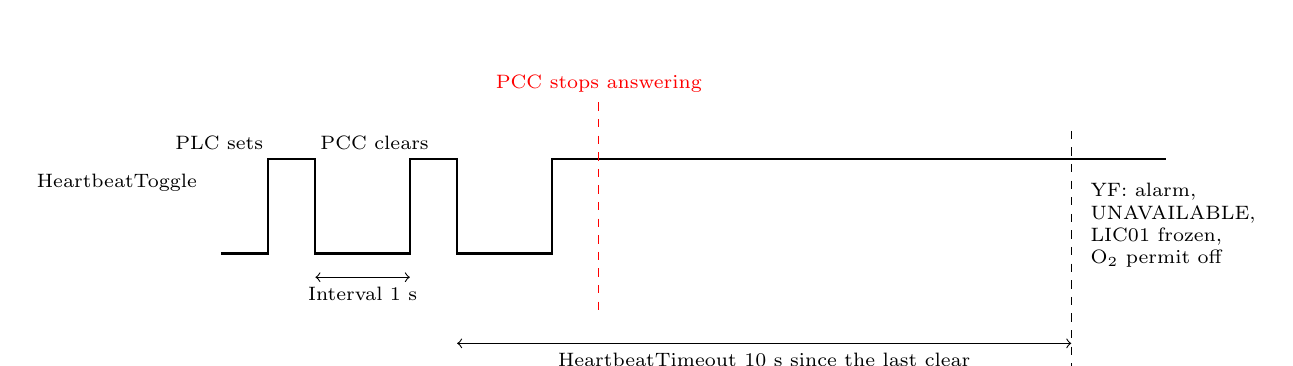
\begin{tikzpicture}[font=\scriptsize, x=6mm, y=6mm]
  \node[anchor=east] at (-0.3,1.5) {HeartbeatToggle};
  \draw[thick] (0,0) -- (1,0) -- (1,2) -- (2,2) -- (2,0) -- (4,0) -- (4,2) -- (5,2) -- (5,0) -- (7,0) -- (7,2) -- (20,2);
  \node[above left] at (1.1,2) {PLC sets}; \node[above right] at (1.9,2) {PCC clears};
  \draw[<->] (2,-0.5) -- node[below] {Interval 1 s} (4,-0.5);
  \draw[dashed, red] (8,3.2) node[above, text=red] {PCC stops answering} -- (8,-1.3);
  \draw[<->] (5,-1.9) -- node[below] {HeartbeatTimeout 10 s since the last clear} (18,-1.9);
  \draw[dashed] (18,2.6) -- (18,-2.6);
  \node[anchor=west, align=left] at (18.2,0.6) {YF: alarm,\\UNAVAILABLE,\\LIC01 frozen,\\O$_2$ permit off};
\end{tikzpicture}
\caption{Heartbeat as implemented in [PLC]: one shared bit, the PLC sets it, the PCC clears it.}
\label{fig:hb}
\end{figure}

\subsection{Operating modes}
The operating modes (Table~\ref{tab:modes}) are selected on the outlet function. A mode sets the
damper opening and, per [FD], the level setpoint of LIC01 and the number of pumps (2 or 3). In [PLC]
the outlet has the mode table with damper positions; the level setpoint is not taken from the mode
yet\open{14}. The number of pumps follows from the flow needed (Section~\ref{sec:count}) instead of from
the mode.

% =====================================================================================================
\section{Functional requirements}
\label{sec:freq}

\subsection{Processes}
\begin{enumerate}[label=P\arabic*, leftmargin=10mm]
  \item The system shall pump sea water into the pen with up to three Framo inlet pumps; normally 2 or
        3 run, depending on the operating mode.
  \item The system shall hold the over-height $\Delta H_\text{avg}$ at the setpoint by setting one common
        speed for all pumps in REMOTE in level control, their share of LIC01's total speed.
  \item The system shall start and stop the pumps in automatic from one Pen Start / Pen Stop command,
        and let the operator start, stop and set the speed of a pump in manual.
  \item While the pen runs, the system shall run only as many pumps as the flow needs, near their
        operating speed, and rotate the running pumps by run time (Section~\ref{sec:count}).
  \item The system shall supervise the link to each Framo controller and react to its loss (HOLD).
  \item The system shall give each oxygen line its permit only while its inlet pump runs in REMOTE
        with a live link (interlock I1).
  \item The system shall present the pump state, the Framo values and alarms, and the levels on the HMI.
\end{enumerate}

\subsection{Inputs}
\begin{table}[htbp]
\centering\small
\caption{Inputs to the inlet functions (details in Tables~\ref{tab:instr} and~\ref{tab:opcua}).}
\label{tab:inputs}
\begin{tabularx}{\textwidth}{@{}P{46mm}P{34mm}L@{}}
\toprule
Input & Source & Used for \\
\midrule
LT01--03, LT21--23 & InletRIO $n$ words 0, 1 & PV of LIC01, display, alarms \\
Pump state flags (7 per pump) & PCC$n$, OPC UA & F4, tracking, hold, start permissive \\
MotorVelocity & PCC$n$, OPC UA & tracking, bumpless transfer, display \\
Framo alarms (11 per pump) & PCC$n$, OPC UA & alarms, info panel \\
HeartbeatToggle & PCC$n$, OPC UA & link supervision \\
Vacuum status (LSL, LSH, V001, V002, air pressure) & PCC$n$, OPC UA & display; overfill alarm\open{11} \\
Drive values (current, power, \ldots) & PCC$n$, OPC UA & info panel \\
24 V field breaker XF05 status & InletRIO $n$ word 4.0 & alarm (it feeds the LT loops) \\
Operator commands and parameters & HMI, OPC UA & Table~\ref{tab:hmi} \\
\bottomrule
\end{tabularx}
\end{table}

\subsection{Outputs}
\begin{itemize}[nosep]
  \item Per pump, to PCC$n$ over OPC UA: Start, Stop, Reset, SpeedSetpoint [rpm], HeartbeatToggle (set).
  \item To the oxygen system: \var{Inlet[i].InletPump.Status.OxyPermit} (permit I1).
  \item To the HMI: states, PV, setpoint, LIC01 output and mode, alarms.
\end{itemize}
The inlet system has no hard-wired outputs; the PLC has no command path to the pumps other than
OPC UA. A lost link therefore always leaves the pump to the PCC (HOLD).

\subsection{Startup and shutdown}
\textbf{PLC start (power-up, download).} Configuration and the level setpoint are retained. The pen
start latch is not retained: after a PLC restart no pump is started automatically. [FD] Tabell~2--3
asks for auto-restart after a power failure, in a sequence to avoid simultaneous inrush currents; this
is not implemented\open{16}. The PLC shows every pump UNAVAILABLE until its PCC has answered the
heartbeat once, so no Start is sent on stale data.

\textbf{Normal start} and \textbf{normal stop}: Figure~\ref{fig:seq}.

\textbf{Pump start while others run.} A pump started (in auto or manual) while another pump is
already in REMOTE does not interrupt automatic control: while it starts its speed counts in LIC01's
total and the pumps in REMOTE give way; it reaches REMOTE at about its share.

\textbf{Emergency stop.} Each PCC has a local E-stop pushbutton acting on the drive's Safe Torque Off;
[EL] 874.001 notes that multiple E-stop actuators are connected in series. Whether the E-stops stop all
three lines, and how the oxygen line is stopped on E-stop through the Heimdall PLC, is to be
confirmed\open{13}. The PCC reports \var{EmergencyStop}; the pump goes to LOCKDOWN (or UNAVAILABLE if it
was not running).

\subsection{Fault identification and recovery}
\label{sec:faults}
\begin{small}
\begin{longtable}{@{}P{30mm}P{34mm}P{50mm}P{38mm}@{}}
\caption{Faults, detection, automatic response and recovery.}\label{tab:faults}\\
\toprule
Fault & Detection & Automatic response & Recovery \\
\midrule
\endfirsthead
\toprule
Fault & Detection & Automatic response & Recovery \\
\midrule
\endhead
\bottomrule
\endfoot
One level transmitter bad & 750-455 status bits $\neq$ 00 (wire break, over-range) for 1~s & Quality alarm; its \emph{pair} drops out of the PV; LIC01 continues on the remaining pairs & Automatic when healthy; the filter restarts at the current value (no dip) \\
Transmitter disabled by operator & Config.Enable FALSE & Pair drops out & Operator enables it \\
All pairs lost & no valid pair & Alarm \emph{Level measurement lost} (LAL01); LIC01 to manual at \var{SafeOutput} 60~rpm (interlock I6) & Back to auto bumplessly when a pair is valid \\
InletRIO $n$ link lost & Modbus TCP \var{CommOK} FALSE & Alarm \emph{InletRIO comm.\ error}; both transmitters of inlet $n$ count as bad, so its pair drops out of the PV (DEC6) & Automatic \\
24 V field breaker XF05 tripped & InletRIO word 4.0 & Alarm; both transmitters of that inlet read bad $\Rightarrow$ pair drops out & Reset XF05 (HMI, DO 0.0) \\
Framo link / heartbeat lost & no clear for 10~s & Alarm \emph{Communication loss}; PLC shows UNAVAILABLE; LIC01 output frozen if the pump was in level control; oxygenation permit off. PCC: HOLD at preset speed & Link back: PCC still in HOLD $\Rightarrow$ operator Reset\open{2}; when REMOTE, LIC01 resumes from the actual speed \\
Pump trip / fault & PCC alarm flags; state LOCKDOWN & Common alarm \emph{Pump $n$ failed}; pump leaves level control; the remaining pumps take over its share in the same cycle (DEC5); if their share stays $\ge$ \var{PumpAddSpeed}, a standby candidate is started; permit off & Fix the fault, operator Reset\open{3}; as a candidate it is started again while the pen runs \\
Start not acknowledged & Start sent, still AVAILABLE after 30~s & Alarm \emph{Start failed}; a candidate is left out of the pump count and another one is started if the share stays high (Section~\ref{sec:count}) & Operator \\
Stop not acknowledged & Stop sent, still in START, REMOTE or HOLD after 30~s & Alarm \emph{Stop failed} & Operator, locally at the PCC \\
Reset not answered & Reset given in HOLD or LOCKDOWN, pump still in that state after $2\times$\var{ResetExpectedTime} (10~s) & Reset withdrawn; warning \emph{Failed to reset} (no acknowledge) & Check the PCC; give Reset again \\
Speed deviation & $|n_\text{SP}-n| >$ \var{SpeedDeviationLimit} (10~rpm) for \var{SpeedDeviationDelay} (30~s), in REMOTE & Alarm \emph{Speed deviation} & Operator; automatic when the pump follows again \\
Vacuum chamber overfill & LSH3$n$ & not implemented (5~s delay in [FD])\open{11} & -- \\
Emergency stop & PCC \var{EmergencyStop} & Pump stops (STO); alarm; LOCKDOWN & Release E-stop, Reset\open{13} \\
LIC01 at its limit & \var{LimitsActive} & Alarm; integral held (anti-windup of \var{Util.PID}) & Automatic \\
Level not held & $|\Delta H_\text{avg}-\mathrm{SP}| >$ the limit for the delay, LIC01 in auto & Alarm \emph{Level deviation high / low} & Operator; automatic when back within the limit \\
\end{longtable}
\end{small}

\subsection{Interlocks}
\begin{small}
\begin{tabularx}{\textwidth}{@{}P{8mm}LP{30mm}P{16mm}@{}}
\toprule
ID & Interlock & Source & In PLC \\
\midrule
I1 & Oxygenation permit line $n$ = PM-3$n$ in REMOTE AND heartbeat OK. & [FD] \S3.2.1, [PID] -100 & \impl \\
I2 & 2oo3 high-high LS7$n$mHH in inlet box $n$ stops PM-3$n$. & [FD] \S3.2.6, [PID] -600 & \notimpl\open{20} \\
I3 & Group start only with the outlet open. & PLC function flow diagram & \notimpl\open{20} \\
I6 & No valid level pair: LIC01 to manual at SafeOutput. & [PID] -400 & \impl \\
-- & Start only when the pump is AVAILABLE and the link is OK. & [FD] Tabell~5 & \impl \\
-- & Emergency stop: Framo E-stop stops the pump (STO); oxygen line to stop. & [FD] Tabell~2, [EL] & partly\open{13} \\
\bottomrule
\end{tabularx}
\end{small}

\subsection{Communication}
\begin{itemize}[nosep]
  \item \textbf{PLC $\leftrightarrow$ Framo PCC$n$:} OPC UA. The PLC is the client (CODESYS Data Sources
        \var{Framo_1..3}); each PCC is a server (TwinCAT TF6100). Signal list: Table~\ref{tab:opcua}.
        Start, Stop and Reset are events acted on at the rising edge\open{4}. The PLC holds Reset TRUE
        from the operator's command until it reads the pump out of HOLD or LOCKDOWN, at most
        $2\times$\var{ResetExpectedTime}; then it withdraws Reset and warns \emph{Failed to reset}.
  \item \textbf{PLC $\leftrightarrow$ InletRIO $n$:} Modbus TCP, function code 23, every 100~ms.
  \item \textbf{HMI $\leftrightarrow$ PLC:} OPC UA (PLC is the server).
\end{itemize}

% =====================================================================================================
\section{Non-functional requirements}
\label{sec:nfreq}

\subsection{Control law and tuning}
LIC01 is a PI controller (CODESYS \var{Util.PID} wrapped in \var{PIDController}):
\[
T(t) = K_p\Big(e(t) + \frac{1}{T_i}\int e\,dt\Big) + Y_\text{offset}, \qquad e = \mathrm{SP} - \Delta H_\text{avg},
\]
the total speed of the pumps in level control, limited to $N\times$(40--130)~rpm and shared as in
Section~\ref{sec:lic}; while the output is at a limit Util.PID adapts the integral to the limited output
(anti-windup). Manual$\to$auto gives \var{RESET} for one cycle (clears the integral and applies $K_p$,
$T_i$) with $Y_\text{offset} = Y_\text{prev} - K_p e$, so the first automatic output is $Y_\text{prev}$
(bumpless); on the operator's manual$\to$auto the setpoint is first set to the PV, so $e = 0$ and
$Y_\text{offset} = Y_\text{prev}$. Auto$\to$manual (\var{LevelController.Status.Manual} rising) sets
\var{LevelController.Command.ManualOutput} $= Y_\text{prev}/N$. In manual Util.PID sets
$Y = Y_\text{manual}$ without its limits; \var{PIDController} therefore limits the manual output to
\var{OutputMin}..\var{OutputMax} (all four controllers), so manual never drives LIC01 below
$N\times40$~rpm. Util.PID applies new $K_p$, $T_i$ only
at a reset: after changing the tuning in auto, give \emph{Auto} once (restart from the current output).

\begin{table}[htbp]
\centering\small
\caption{LIC01 start values.}
\label{tab:tuning}
\begin{tabularx}{\textwidth}{@{}lP{24mm}P{30mm}L@{}}
\toprule
Parameter & [PLC] & [FD] Tabell 8 & Comment \\
\midrule
$K_p$ & 1350 total rpm/m & P = 0.5 / 1 / 2 for 1 / 2 / 3 pumps & = the former 450 rpm/m per pump with 3 pumps ($\approx$ [FD] P = 1: 90 rpm over 0.20 m). With the total output one set holds for every pump count (DEC5) \\
$T_i$ & 60 s & 600 s & 600 s gives a closed loop of about 16 min [DES]; 60 s tested\decided{4} \\
$T_d$ & 0 & -- & PI \\
Output & $N\times$40--130 rpm (total) & 40--130 rpm & per pump 40--130 rpm \\
PV scaling & m & 0--20 cm & \\
Margins (worst case O-35, 3 pumps) & PM 76$^\circ$, GM 13.2 dB, $1/\omega_c$ = 100 s & -- & [DES] \S7, dead time 2.5$\theta$ \\
\bottomrule
\end{tabularx}
\end{table}

\textbf{Simulator tests} (PFC200 against CasRioSim/CasFramoSim, O-35, 3 pumps, $K_p$ 450 per pump, $T_i$ 60~s, before the sharing):
\begin{itemize}[nosep]
  \item start-up: pumps reach REMOTE at about 87~rpm, take-over bumpless;
  \item setpoint step +2~cm: settles in about 100~s, no overshoot;
  \item one of three pumps lost: the level dips 3.4~cm; the pump rejoining gives 2.7~cm overshoot. There
        is no feed-forward on the number of pumps, and the integral winds up against 130~rpm while two
        pumps carry the load.
\end{itemize}
\textbf{Baseline} (2026-10-22, same rig): pump 3 out $\Rightarrow$ level 6.0 $\to$ 3.0~cm, about 4~min back;
pump 3 restart $\Rightarrow$ 9.1~cm, mostly during its START (its own preset speed while the others still
ran fast). \textbf{Change} (DEC5): the output is the total speed, shared by the pumps in REMOTE, so a
trip or a start is compensated in the same cycle. An I-PD form would avoid the setpoint kick on mode
changes.

\textbf{Live test} (2026-10-22, PFC200 10.1.2.41 on \var{main} after Reset Origin, CAS plant simulator
10.1.2.150, O-35):
\begin{itemize}[nosep]
  \item Pen Start from a drained pen ($-3.4$~cm): Starting $\to$ Running when the pumps reached REMOTE;
        LIC01 tracked the summed speed (260~rpm) and handed over at 85.5~rpm per pump (bumpless); level
        peak 6.6~cm (0.6~cm overshoot), settled at 6.1~cm in about 2.5~min with three pumps at 74~rpm.
  \item Pump stopped by the pump count (test values \var{PumpTargetSpeed} 115~rpm, delay 60~s): the pump
        with the most running days stopped, the other two took its share in the same cycle; level dip
        6.0 $\to$ 5.2~cm, back to 6.3~cm; two pumps at about 112~rpm, no flapping.
  \item Rotation (test value \var{PumpCycleTime} 2~min): the standby started first and the old pump
        stopped once the new one was in REMOTE; level 5.1--7.1~cm during each handover (register
        IN-31). With a short cycle the rotations follow each other, as every running pump has passed it.
  \item Commands: O$_2$ Start with the pen Stopped was refused (\var{CommandRejected}); all pulses were
        cleared by the PLC in the same scan.
  \item Not yet tested: pump trip, level and speed deviation alarms, RIO link loss with the new code.
\end{itemize}

\textbf{Small setpoints.} O-60 and S-75 use a 0.5~cm setpoint, against about 1~mm resolution of the
over-height, $\pm$6~mm combined transmitter uncertainty and waves up to $H_s$ = 2~m. Whether this is
controllable, and with what filter, is open\open{7}.

\subsection{Cycle times and tasks}
\begin{table}[htbp]
\centering\small
\caption{Tasks and timing ([PLC] Task Configuration of PFC200\_Sim).}
\label{tab:tasks}
\begin{tabularx}{\textwidth}{@{}P{30mm}P{18mm}L@{}}
\toprule
Task & Cycle & Inlet content \\
\midrule
\var{Task} & 20 ms & \var{Main}: InletSupervisor (LIC01, sequence), InletControl[0..2] (pump control, heartbeat, InletSensors), PenControl (PV); \var{IO_Processing} (InletRIO masters) \\
\var{OPC_Processing} & 50 ms & \var{FramoDataProcessing}: maps Framo\_$n$ to/from GVLMain \\
\var{DatasourcesTask} & 50 ms & OPC UA client (Data Sources) to the PCCs \\
Modbus TCP poll & 100 ms & InletRIO $n$, FC23 \\
\bottomrule
\end{tabularx}
\end{table}
A level reading reaches LIC01 two \var{Task} cycles after it is read; the speed setpoint reaches the
PCC within some tenths of a second plus the OPC UA publishing time. This is small against the level
loop's dead time of about 2~s and time constant of 28--40~s [DES]. Task watchdogs are disabled in the
test application\open{23}.

\subsection{Signal resolution and filtering}
\begin{itemize}[nosep]
  \item \textbf{750-455:} value in bits 14..4 (0..2047), bits 3..2 reserved, bits 1..0 diagnostics;
        20~mA = \texttt{0x7FF0}\decided{2}. On the 0--2~m span one step is 0.98~mm; the over-height, the
        difference of two readings, moves in steps of about 1~mm. The PLC scales
        $\text{Raw}\cdot(\text{Max}-\text{Min})/32760 + \text{Min}$ (20~mA reads 99.98\,\% of span).
  \item \textbf{Transmitter accuracy:} inside $\pm$2~mm (radar), outside $\pm$4~mm (pressure, 0.2\,\%
        of an assumed 2~m full scale)\open{18}.
  \item \textbf{Filter:} 2nd-order Butterworth per pair, $f_c$ = 0.05~Hz, bilinear with pre-warping,
        sample time = task cycle read from the runtime, LREAL coefficients. A 1~cm step reaches 63\,\% in
        5.6~s with 4\,\% overshoot; 4--10~s waves are attenuated by about 19~dB [DES]. The filter
        restarts at the current value when a pair becomes valid.
  \item The per-transmitter filters (\var{FilterFc} 0.05~Hz) are for display only.
  \item \textbf{Signal direction:} raw 0 (4~mA) is assumed to be the lowest level; to be read in the
        transmitters. Inside and outside must agree, or the sign of LIC01 is wrong\open{18}.
\end{itemize}

\subsection{Alarm functions}
Alarm states are handled by \var{AlarmManagement} (raised on the condition, acknowledged on the
rising edge of the acknowledge bit). [AL] defines no priorities or acknowledgement classes; the
column Class is a proposal (A = alarm, operator action; W = warning; N = notification only)\open{21}.

\begin{small}
\begin{longtable}{@{}P{34mm}P{46mm}P{9mm}P{34mm}P{20mm}@{}}
\caption{Alarms of the inlet system ([FD] Tabell 7 and 9, [AL], [PLC]). Per pump $n$ = 1..3 unless
noted.}\label{tab:alarms}\\
\toprule
Alarm & Condition & Class & Action & PLC \\
\midrule
\endfirsthead
\toprule
Alarm & Condition & Class & Action & PLC \\
\midrule
\endhead
\bottomrule
\endfoot
Communication loss pump $n$ & PCC has not cleared HeartbeatToggle for 10~s & A & UNAVAILABLE; LIC01 frozen; O$_2$ line $n$ stops & \impl \\
Start of pump $n$ failed & Start sent and still AVAILABLE after StartupTime (30~s) & A & none & \impl \\
Stop of pump $n$ failed & Stop sent and still in START, REMOTE or HOLD after ShutdownTime (30~s) & A & none & \impl \\
Failed to reset pump $n$ & Reset given in HOLD/LOCKDOWN, no state change within $2\times$ResetExpectedTime (10~s); clears when the pump leaves HOLD/LOCKDOWN or on a new Reset & W (auto-ack) & Reset withdrawn & \impl \\
Pump $n$ failed (common) & any of DriveError, DriveCommunication, DriveNotInRemote, MotorTemperature, EmergencyStop, DCUndervoltageError, PumpStopped, UPSSupplyError, EmergencyRunMode & A & shown on info panel & \impl\open{10} \\
Individual Framo alarms & each flag above, own alarm & A & logged & \impl \\
Pump $n$ low / high power & LowPower / HighPower from PCC; not in the common alarm & N (auto-ack) & none, notification only [FD] & \impl \\
Speed deviation pump $n$ & $|n_\text{SP}-n| >$ \var{SpeedDeviationLimit} (10~rpm) for \var{SpeedDeviationDelay} (30~s), in REMOTE (\var{Inlet[i].InletPump.Alarm.SpeedDeviation}) & W & none & \impl \\
Vacuum overfill line $n$ & LSH3$n$ for 5~s (configurable) & A & none & \notimpl\open{11} \\
Emergency stop activated & EmergencyStop from PCC (hard-wired \TBD) & A & pump stops & via Framo\open{13} \\
Level deviation high / low & $\Delta H_\text{avg}$ more than \var{LevelDeviationLimit} (0.02~m) above / below SP for \var{LevelDeviationDelay} (5~min), LIC01 in auto (\var{Pen.Alarm.LevelDeviationHigh}, \var{.LevelDeviationLow}) & A & none & \impl \\
Low level in pen & $\Delta H_\text{avg} <$ \TBD{} for \TBD{} s & A & none & \notimpl\open{8} \\
High level in pen & $\Delta H_\text{avg} >$ \TBD{} for \TBD{} s & A & none & \notimpl\open{8} \\
Level transmitter fault (LT01--03, LT21--23) & 750-455 status bits $\neq$ 00 for 1~s & W & pair drops out of PV & generic quality alarm\open{8} \\
Level measurement lost (LAL01) & no valid pair (pen) & A & LIC01 at SafeOutput & \impl \\
LIC01 output at limit / overflow & \var{LimitsActive}, \var{Overflow} (pen) & W & none & \impl \\
InletRIO $n$ communication error & Modbus \var{CommOK} FALSE & A & pair $n$ drops out of the PV & \impl \\
InletRIO $n$ field power & XF05 tripped & A & LTs of inlet $n$ lost & \impl \\
\end{longtable}
\end{small}

\subsection{Parameters}
All parameters are written from the HMI and retained: \var{Main.UpdateRetain} keeps them in step
with \var{GVLRetain}. Defaults from \var{ConfigValues} apply on a fresh download (rev~B added fields to
\var{PenConfigDUT}: download with Reset Origin).

\begin{small}
\begin{longtable}{@{}P{58mm}P{24mm}P{10mm}P{55mm}@{}}
\caption{Configurable parameters of the inlet system.}\label{tab:params}\\
\toprule
Parameter & Default & Unit & Meaning \\
\midrule
\endfirsthead
\toprule
Parameter & Default & Unit & Meaning \\
\midrule
\endhead
\bottomrule
\endfoot
\var{PenConfig.LevelController.Kp} & 1350 & rpm/m & LIC01 gain on the total speed \\
\var{PenConfig.LevelController.Ti} & 60 & s & integral time (new value takes effect at the next start or manual$\to$auto) \\
\var{PenConfig.LevelController.Td} & 0 & s & derivative time \\
\var{PenConfig.LevelController.MinOutput} / \var{MaxOutput} & 40 / 130 & rpm & speed range per pump (LIC01: $\times N$) \\
\var{PenConfig.LevelController.SafeOutput} & 60 & rpm & speed per pump with no valid level pair \\
\var{PenConfig.LevelDeviationLimit} / \var{LevelDeviationDelay} & 0.02 / 5 & m / min & level deviation alarms; limit 0 = off \\
\var{PenConfig.PumpTargetSpeed} & 85 & rpm & stop a pump when the others would run at or below this; 0 = never \\
\var{PenConfig.PumpAddSpeed} & 115 & rpm & start a pump when the share is at or above this; above \var{PumpTargetSpeed}; 0 = never \\
\var{PenConfig.PumpRemoveDelay} / \var{PumpAddDelay} & 15 / 2 & min & how long the stop / start condition must hold \\
\var{PenConfig.PumpCycleTime} & 24 & h & time in REMOTE before a standby takes over; 0 = no rotation \\
\var{InletConfig[i].InletPump.Enable} & TRUE & & pump $i$ takes part in the pump count and rotation \\
\var{Pen.Command.LevelSetpoint} & 0.06 & m & over-height setpoint (O-35) \\
\var{LevelInsideConfig[i]}: Enable, MinValue, MaxValue & TRUE, 0, 2.0 & m & LT0$i$ in use and range \\
\var{LevelInsideConfig[i]}: FilterFc, QualityEnabled & 0.05, TRUE & Hz & display filter; quality alarm \\
\var{LevelOutsideConfig[i]}: as inside & as inside & & LT2$i$ \\
\var{OverHeightConfig[i]}: Enable, FilterFc & TRUE, 0.05 & Hz & pair in use; cut-off of the pair's filter (0 = off) \\
\var{InletConfig[i].HeartbeatInterval} & 1 & s & PLC sets the bit this long after the PCC cleared it \\
\var{InletConfig[i].HeartbeatTimeout} & 10 (DUT 5) & s & link-loss detection \\
\var{InletConfig[i].StartupTime} / \var{ShutdownTime} & 30 / 30 & s & start / stop failed alarms \\
\var{InletConfig[i].SpeedDeviationLimit} / \var{SpeedDeviationDelay} & 10 / 30 & rpm / s & speed deviation alarm in REMOTE; limit 0 = off \\
\var{InletConfig[i].ResetExpectedTime} & 5 & s & expected PCC response to Reset (OPC UA round trip $\approx$4.6~s); warning \emph{Failed to reset} after $2\times$ \\
\var{InletRIOConfig[i]}: IP, Port & sim: 10.1.2.150, 5121--5123 & & coupler address (site plan \TBD) \\
Data sources \var{Framo_1..3} & per project & & OPC UA endpoint of each PCC \\
Not yet defined: L/H level limits and delays, speed deviation limit, vacuum overfill delay (5~s), mode table SP & \TBD & & \open{8}\open{9}\open{11}\open{14} \\
\end{longtable}
\end{small}

\subsection{Interfaces: instruments and actuators}
{\setlength{\tabcolsep}{1.4pt}\begin{instrumenttable}{Instruments, actuators and PLC functions of the inlet system ([PID], [EL], [DES]). Use: C = control, M = monitor, A = alarm.}
\label{tab:instr}
LT01--03 & Level inside the pen, at inlet $n$; VEGAPULS radar\open{18} & Gooseneck, inlet $n$ & 4--20 mA 2-wire, InletRIO $n$ -R1-106 ch1, word 0 & 0--2 m & 0.98 mm; $\pm$2 mm & C, M, A \\
LT21--23 & Sea level outside the pen, at inlet $n$; submersible pressure probe & Outside the collar, inlet $n$ & 4--20 mA 2-wire, InletRIO $n$ ch2, word 1 & 0--2 m (assumed) & 0.98 mm; $\pm$4 mm & C, M, A \\
LDY01--03 & Over-height of pair $n$, filtered & PLC & computed & 0--0.20 m & $\approx$1 mm & C \\
LY01 & Mean over-height of valid pairs (PV) & PLC & computed & 0--0.20 m & -- & C, A \\
LIC01 & Level controller, PI & PLC & output to SY31--33 & 40--130 rpm & -- & C \\
LAL01 & Level measurement lost & PLC & alarm & -- & -- & A \\
PM-31--33 & Framo SR2000 inlet pump, rim motor 60 kW & Intake $n$ & via PCC$n$ (ACS880) & 40--130 rpm, 20\,000 m$^3$/h & -- & actuator \\
SC31--33 & Framo pump controller CX8200 + ACS880-31-105A-3 & PCC$n$ & OPC UA server & -- & -- & -- \\
SY31--33 & Speed setpoint to pump $n$ & PLC $\to$ PCC$n$ & OPC UA SpeedSetpoint & 40--130 rpm & REAL & C \\
SI31--33 & Actual pump speed & PCC$n$ & OPC UA MotorVelocity & 0--130 rpm & REAL & C, M \\
HS31--33 & Start / Stop / Reset pump $n$ & PLC $\to$ PCC$n$ & OPC UA events & -- & -- & C \\
YI31--33 & Pump state & PCC$n$ & OPC UA 7 flags & 7 states & -- & C, M \\
UA31--33 & Pump alarms (11 flags) & PCC$n$ & OPC UA alarms & -- & -- & A \\
KY31--33 & Heartbeat & PLC $\leftrightarrow$ PCC$n$ & OPC UA BOOL & -- & -- & C, A \\
LSL31--33 & Vacuum chamber low level (air evacuated) & TV-3$n$ & OPC UA (Framo LSL01) & on/off & -- & M \\
LSH31--33 & Vacuum chamber high level (overfill) & TV-3$n$ & OPC UA (Framo LSH02) & on/off & -- & A\open{11} \\
PT31--33 & Compressed air pressure to ejector & Air line, inlet $n$ & OPC UA analog & Framo range & REAL & M \\
XV31A--33A & Air valve to ejector EJ-3$n$ & Inlet $n$ & status OPC UA (V001?) & open/closed & -- & M\open{11} \\
XV31B--33B & Vacuum break (vent) valve & TV-3$n$ & status OPC UA (V002?) & open/closed & -- & M\open{11} \\
E-stop PCC$n$ & Local emergency stop, STO & PCC$n$ door & OPC UA EmergencyStop & on/off & -- & A\open{13} \\
YA30 (n) & 24 V field breaker XF05 tripped (LT supply) & RIO $n$ cabinet & InletRIO $n$ DI word 4.0 & on/off & -- & A \\
\end{instrumenttable}}

\subsection{Interfaces: OPC UA signals to and from the Framo controllers}
Per pump $n$ the PLC uses the Data Source \var{Framo_n}; the GVL side is \var{GVLMain.Inlet[n-1].InletPump}.
Direction is seen from the PLC (R = read, W = written).

\begin{small}
\begin{longtable}{@{}P{52mm}P{20mm}P{7mm}P{36mm}P{32mm}@{}}
\caption{OPC UA signal list, PLC $\leftrightarrow$ Framo PCC$n$ ([FRAMO] rev.~B, [FD] Tabell 6, [PLC]
FramoDataProcessing).}\label{tab:opcua}\\
\toprule
Signal (Data Source name) & Type & Dir. & Use in PLC & Remark \\
\midrule
\endfirsthead
\toprule
Signal (Data Source name) & Type & Dir. & Use in PLC & Remark \\
\midrule
\endhead
\bottomrule
\endfoot
MotorVelocity (+ ValueRange Low/High) & AnalogValue & R & tracking, bumpless transfer, speed indication & range written by Framo?\open{19} \\
MotorFrequency, MotorCurrent, MotorPower, MotorVoltage, MotorTorque, PowerConsumptionCounter, DCLinkVoltage, VSDHeatSinkTemperature, VSDOperatingDays & AnalogValue & R & info panel & [FRAMO]: PowerConsumtionCounter \\
MotorRunningDays & AnalogValue & R & info panel; run-time order of pumps (\var{SortSequence}) for the pump count and rotation & \\
DriveError, DriveCommunication, DriveNotInRemote, MotorTemperature, EmergencyStop, DCUnderVoltageError, PumpStopped, UPSSupplyError, EmergencyRunMode & Alarm & R & own alarm each; common alarm & \\
LowPower, HighPower & Alarm & R & notification (auto-ack), not in the common alarm & \\
PumpStateUnavailable, \ldots Available, Start, Stop, Remote, Hold, Lockdown & Event & R & \var{InletPump.State} (first TRUE flag) & \\
Start, Stop, Reset & Event & W & commands, rising edge & \open{3}\open{4} \\
SpeedSetpoint & AnalogValue & W & LIC01 output in REMOTE, else actual speed or 0 & [FRAMO], [FD]: Velocity\-Setpoint\open{19} \\
HeartbeatToggle & BOOL & R/W & PLC sets, PCC clears & \open{1} \\
HeartbeatInterval, HeartbeatElapsed & TIME & -- & not mapped & \open{1} \\
PressureCompressedAir, LevelSwitchLSL01, LevelSwitchLSH02, StatusV001, StatusV002 & Analog / BOOL & R & vacuum system status & not in [FRAMO] / [FIL]\open{11} \\
\end{longtable}
\end{small}

\subsection{HMI operator functions}
\begin{table}[htbp]
\centering\small
\caption{Operator functions for the inlet system (PLC variables in [PDS] Table ``Commands'').}
\label{tab:hmi}
\begin{tabularx}{\textwidth}{@{}P{46mm}P{52mm}L@{}}
\toprule
Function & PLC variable & Note \\
\midrule
Pen Start / Pen Stop & \var{Pen.Command.Start}, \var{.Stop}; shows \var{Pen.Status.State}, \var{.Ready}, \var{.CommandRejected} & pulses; Start only when Ready; starts the enabled pumps in auto \\
Oxygen Start / Stop & \var{Pen.Command.OxygenStart}, \var{.OxygenStop}; shows \var{Pen.Status.OxygenOn} & pulses; enabled lines follow their inlet pumps \\
Pump count and rotation & \var{InletConfig[i].InletPump.Enable}; shows \var{PenInletSupervisor.PumpsWanted}, \var{.PumpRotationActive} & take a pump out of the count without manual \\
Level setpoint & \var{Pen.Command.LevelSetpoint} & m; from the mode in future\open{14} \\
LIC01 auto / manual, manual output & \var{LevelController.Command.Manual}, \var{.Auto} (pulses; mode in \var{.Status.Manual}), \var{.ManualOutput} & rpm per pump \\
Pump auto / manual & \var{Inlet[i].InletPump.Command.Auto}, \var{.Manual} (pulses; mode in \var{.Status.Manual}) & default auto \\
Pump start / stop / speed in manual & \var{Inlet[i].InletPump.Command.Start}, \var{.Stop}, \var{.Setpoint} & speed used in REMOTE \\
Reset pump (HOLD, LOCKDOWN) & \var{Inlet[i].InletPump.Command.Reset} & pulse, accepted only in HOLD or LOCKDOWN; the PLC clears it and holds the PCC's Reset until it sees the state change. HMI button per pump\open{24} \\
Enable/disable transmitter or pair & \var{...LevelInsidePen.Config.Enable}, \var{...PenOverHeight.Config.Enable} & takes a pair out of the PV \\
Info panel per pump & \var{Inlet[i].InletPump.Input.*}, \var{.State} & [FD] Figur 3 \\
Alarm list and acknowledgement & \var{*.Alarm.*}, \var{*.AlarmAck.*} & classes \TBD\open{21} \\
Parameters (Table~\ref{tab:params}) & \var{GVLMain.PenConfig}, \var{InletConfig}, \ldots & access level \TBD \\
\bottomrule
\end{tabularx}
\end{table}

% =====================================================================================================
\section{Open issues and decisions}
\label{sec:open}

\subsection{Open issues}
Each item names the sources that disagree and, where there is one, a proposal. ``Framo'' items need
agreement with the supplier.

\begin{small}
\begin{enumerate}[label=\textbf{OI\arabic*}, leftmargin=12mm, itemsep=0.5mm]
  \item \textbf{Heartbeat baseline.} PLC: one shared BOOL, PLC sets / PCC clears, neither side waits after
        connect, interval 1~s, timeout 10~s (DUT default 5~s). [FRAMO] rev.~B: HeartbeatToggle with
        HeartbeatInterval and HeartbeatElapsed. [FD]: INT counter 0--32767. Agree one with Framo, incl.\
        the PCC's own timeout and whether the PLC writes Interval.
  \item \textbf{HOLD $\to$ REMOTE.} [FD] requires an operator Reset; [FRAMO] rev.~B returns to REMOTE
        automatically when the heartbeat is back. The PLC works either way: it follows the state the PCC
        reports (LIC01 frozen while in HOLD, bumpless resume in REMOTE) and sends Reset only when the
        operator gives it. Open with Framo: which behaviour the PCC implements, and whether the PCC's own
        panel also has a local Reset.
  \item \textbf{LOCKDOWN exit and Reset.} [FD]: operator Reset after the fault is fixed. [FRAMO]:
        LOCKDOWN ends with ``sequence end'' to UNAVAILABLE, no Reset. What Reset does (all alarms? edge?)
        is not described (Framo review comment).
  \item \textbf{Stop and command semantics.} [FRAMO] rev.~B accepts Stop only in REMOTE (not in START or
        HOLD). The PLC sends Stop in any state and raises Stop failed for START, REMOTE and HOLD. Are Start/Stop/Reset
        edge- or level-triggered?
  \item \textbf{LIC01 parameter sets.} \emph{Closed in rev~B} by DEC5: with the total output the loop gain
        does not depend on the pump count; one set ($K_p$ 1350 total rpm/m, $T_i$ 60~s). [FD] Tabell~8 to
        be updated.
  \item \textbf{Pump-count transients.} \emph{Closed in rev~B} by DEC5 (sharing of the total); to be
        confirmed in the simulator. I-PD against setpoint kick still to consider.
  \item \textbf{0.5~cm setpoint (O-60, S-75).} Controllable with $\approx$1~mm resolution, $\pm$6~mm
        uncertainty and waves? Decide the setpoint, filter and acceptance criterion.
  \item \textbf{Pen level alarms.} Deviation alarms high / low implemented (DEC8; 0.02~m, 5~min, to be
        confirmed). Low and high level alarms of [FD] Tabell 9 / [AL] are not in the PLC; limits and
        delays TBD. The per-transmitter fault exists only as the generic
        quality alarm; map it to the [AL] text per tag.
  \item \textbf{Speed deviation alarm} (in REMOTE) of [FD] Tabell 7: implemented in rev~B (10~rpm, 30~s, to be
        confirmed against Framo's speed response).
  \item \textbf{LowPower / HighPower.} \emph{Closed in rev~B}: removed from \var{PumpCommonError}; their own
        alarms are notifications without acknowledge, as [FD].
  \item \textbf{Vacuum system.} Alarms not implemented (\var{VacuumSystemAlarmDUT} is empty; LSH overfill
        with 5~s delay). The vacuum signals are not in [FRAMO] or [FIL]. Tag mapping to confirm: Framo
        LSL01/LSH02/V001/V002 vs [PID] LSL3$n$/LSH3$n$/XV3$n$A/B vs [FD] LSL31/LSH32/XV31/XV32.
  \item \textbf{Flow figures.} [FD] Tabell 10 O-35 = 34\,000~m$^3$/h; [DES] maximum 27\,000~m$^3$/h;
        3 pumps $\times$ 20\,000~m$^3$/h rated. Framo comment: ``26\,000 ok for emergency mode?''. Align.
  \item \textbf{Emergency stop.} Do the Framo E-stops (in series, [EL] 874.001) stop all three lines?
        How is oxygenation stopped on E-stop through the Heimdall PLC (no E-stop input wired today)?
        [FD] alarm ``Nødstopp aktivert'' is HOLD.
  \item \textbf{Setpoint from operating mode.} [FD]: LIC01 setpoint chosen from the mode, with manual
        override. PLC: operator-entered setpoint only; the outlet mode table has damper positions only.
  \item \textbf{Number of pumps and rotation.} Implemented in rev~B (DEC7, Section~\ref{sec:count}):
        stop and start by the share against \var{PumpTargetSpeed} / \var{PumpAddSpeed}, rotation by run
        time after \var{PumpCycleTime}, next pump when a start fails. Still open: [FD]'s warning when a
        pump has been idle too long; thresholds, delays and cycle time to be confirmed with Framo (start
        and stop wear, minimum run time); the level swing of about $\pm$1~cm during a rotation handover
        (live test 2026-10-22, register IN-31); \var{NumberOfInletsToRun} unused.
  \item \textbf{Auto-restart and start order.} [FD] Tabell 2--3: restart after power failure in a
        sequence (2a/2b/2c). PLC: pen start latch not retained; Pen Start sends Start to all pumps at
        once.
  \item \textbf{InletRIO link loss.} \emph{Closed in rev~B} by DEC6: the pair is invalid while its RIO
        has no communication (tested in the simulator 2026-10-22).
  \item \textbf{Level transmitters.} Signal direction (4~mA = lowest level?) to be read in the sensors;
        inside model VEGAPULS C21 ([DES]) vs C22 ([PID] loop sheet); outside type and 2~m full scale
        assumed.
  \item \textbf{Framo interface details.} Names differ (SpeedSetpoint vs VelocitySetpoint,
        DCUnderVoltageError, PowerConsumptionCounter); is the MotorVelocity range written by Framo?
        Hardware CX8190 ([FRAMO]) vs CX8200 ([EL]); pump SX1000 ([EL]) vs SR2000 ([FD]).
  \item \textbf{Interlocks from other systems.} 2oo3 LS7$n$mHH trip of PM-3$n$ (I2) and ``group start only
        with the outlet open'' (I3) are not in the PLC.
  \item \textbf{Alarm classes.} [AL] has no priority or acknowledgement class; define them.
  \item \textbf{Framo dynamics and preset speeds.} Speed response $T_p$ (10~s assumed), START preset
        speed (88~rpm assumed), HOLD safe speed and ramp rates: to be given by Framo.
  \item \textbf{Platform.} Task watchdogs disabled in the test application; IP plan and network
        drawing missing ([PID] C3).
  \item \textbf{Operator Reset on the HMI.} A Reset button per inlet pump (enabled in HOLD and LOCKDOWN,
        with confirmation) is in review for the test HMI (heimdall-cas-hmi); the production HMI needs the
        same function.
\end{enumerate}
\end{small}

\subsection{Decisions}
\begin{small}
\begin{enumerate}[label=\textbf{DEC\arabic*}, leftmargin=12mm, itemsep=0.5mm]
  \item 2026-10-15 (PLC, in review): PV = mean of the per-pair filtered $\Delta H_i$ over the valid pairs;
        a lost transmitter drops its pair ([FD] \S3.2.2).
  \item 2026-10-07: 750-455 word layout confirmed by WAGO (value in bits 14..4, 0..2047).
  \item 2026-10-15 (PLC, in review): no valid pair $\Rightarrow$ alarm LevelMeasurementLost and LIC01 in
        manual at SafeOutput (60~rpm), bumpless return.
  \item 2026-10-13: LIC01 start value $T_i$ = 60~s instead of 600~s, from the design basis and the
        simulator test; to be confirmed at commissioning.
  \item 2026-10-22: LIC01's output is the total speed of the pumps in level control; the pumps in REMOTE
        share it after the actual speed of the others in level control. $K_p$ 450 per pump $\to$ 1350
        total; per-pump limits, \var{SafeOutput} and manual output scaled by $N$ (IN-05, IN-07).
  \item 2026-10-22: InletRIO $n$ link lost $\Rightarrow$ both transmitters of inlet $n$ bad, its pair
        drops out of the PV (IN-19).
  \item 2026-10-22: automatic pump count and rotation (Section~\ref{sec:count}): candidates = Enable, auto,
        not UNAVAILABLE / LOCKDOWN; start all at Pen Start, then reduce; settings retained in
        \var{PenConfig} (IN-15).
  \item 2026-10-22: level deviation alarms high / low with LIC01 in auto, limit and delay retained in
        \var{PenConfig} (IN-09).
\end{enumerate}
\end{small}

\end{document}
